\chapter{Implementarea sistemului}

\section{Securitate}

Aplicația este securizată din două perspective: taskage-core implementează o componentă personalizată de rută privată, în timp ce endpoint-urile REST expuse de către componenta taskage-core sunt securizate utilizând modulul de securitate pus la dispoziție de către Spring, anume Spring Security.

Ruta privată a modulului front-end, observabilă în figura 4.1, primește ca prop rolul care poate accesa ruta respectivă pentru a putea utiliza componenta în contextul oricărui rol. Aceasta folosește un hook de tip useEffect pentru a detecta schimbarea paginii și a utilizatorului logat. Pentru oricare din aceste schimbări, încarcă un ecran de loading până verifică accesul, apoi, după ce metoda checkAccess determina asincron răspunsul, identifică dacă utlizatorul nu are acces la pagină pentru că nu este logat sau pentru că rolul său nu are privilegii la pagina respectivă. Dacă accesul este oferit, se poate randa un outlet în care să se afișeze pagina cerută, altfel utilizatorul este redirecționat către o pagină cu mesaj sugestiv, precum cel din figura 4.2.

\begin{figure}[hbtp]
	\begin{lstlisting}[frame=single]
	const PrivateRoute = observer(
	  ({ allowedAuthRole }: { allowedAuthRole: String }) => {
	    const location = useLocation();
	    const [isAllowed, setIsAllowed] = useState(false);
	    const [loading, setLoading] = useState(true);
	    const [navigateToRoute, setNavigateToRoute] = useState<string>("");
	
	    useEffect(() => {
	      const checkAccess = async () => {
	        if (userStore.currentUser) {
	          const currentUser = userStore.currentUser;
	          if (currentUser.user.authRole === allowedAuthRole) {
	            setIsAllowed(true);
	          } else {
	            setNavigateToRoute(UNAUTHORIZED_ACCESS_LINK);
	          }
	        } else {
	          setNavigateToRoute(NOT_AUTHENTICATED_LINK);
	        }
	        setLoading(false);
	      };
	
	      checkAccess();
	    }, [userStore.currentUser, location]);
	
	    return loading ? (
	      <Spin />
	    ) : isAllowed ? (
	      <Outlet />
	    ) : (
	      <Navigate to={navigateToRoute} replace />
	    );
	  }
	);
	
	export default PrivateRoute;
	\end{lstlisting}
	\caption{Componenta PrivaterRoute}
\end{figure}

 \begin{figure}[ht]
	\centering
 	 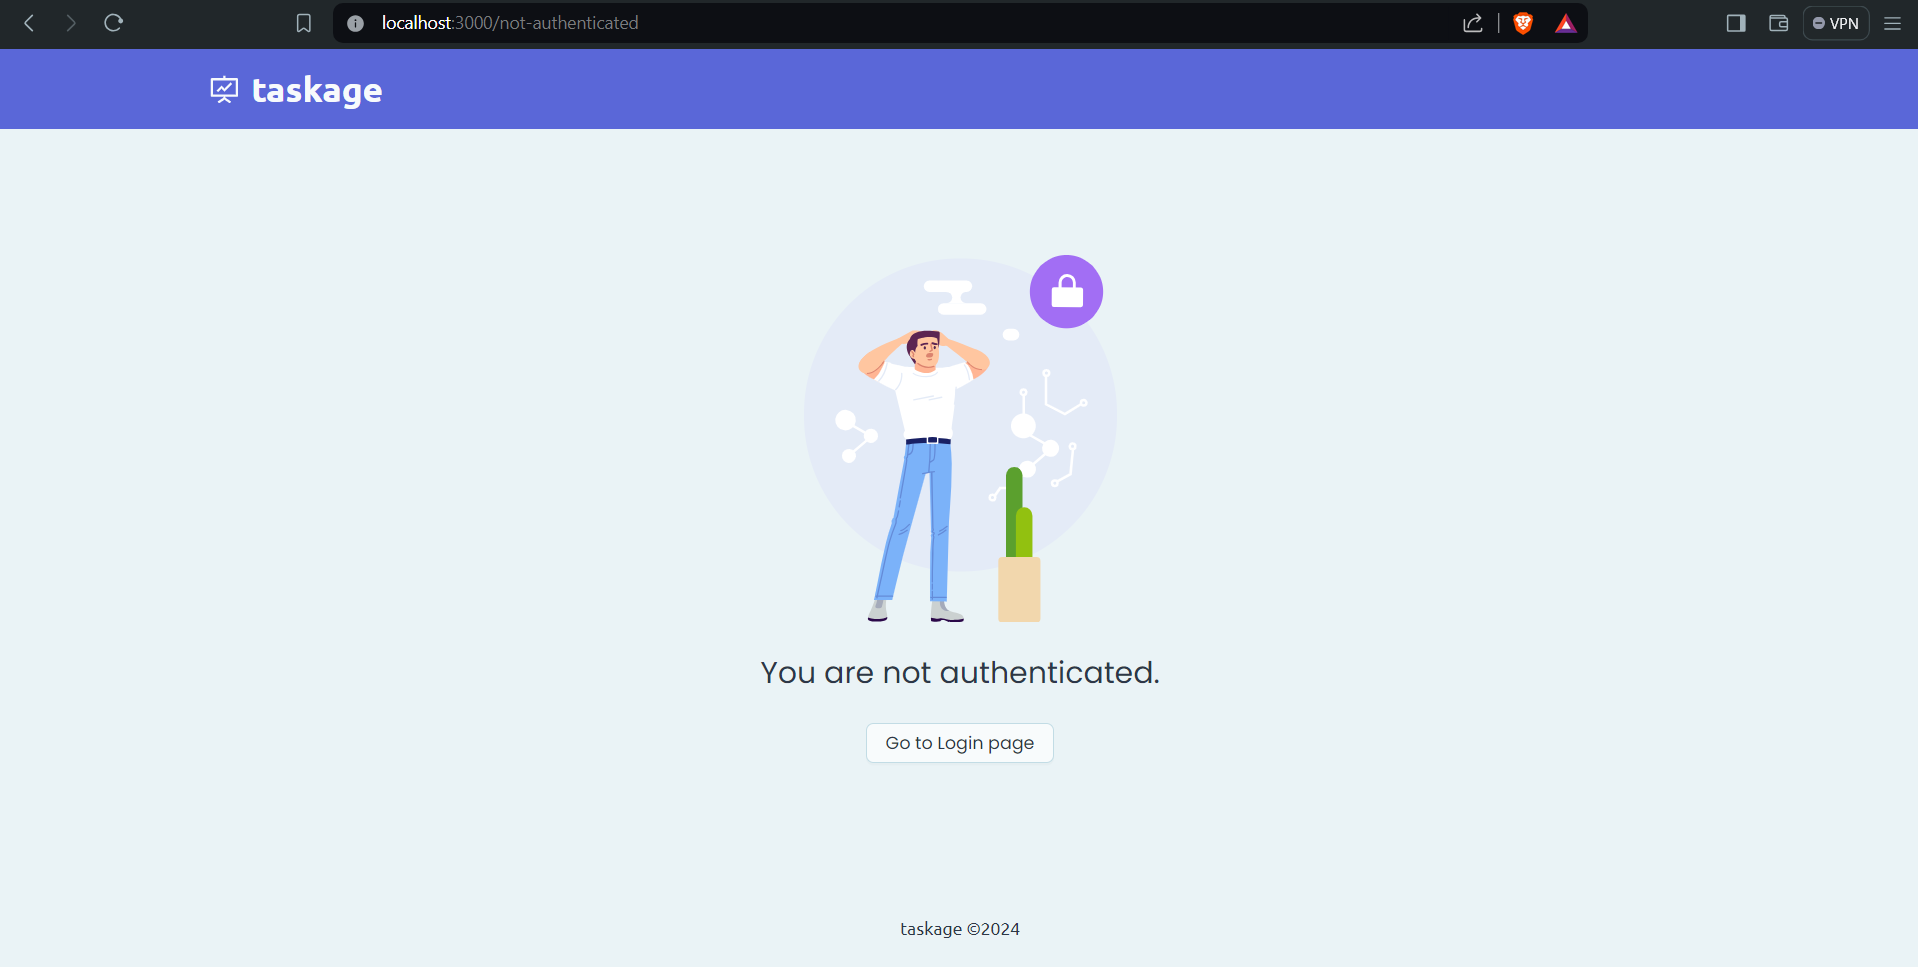
\includegraphics[width=0.8\linewidth]{not-authenticated.png}
	\caption{Pagina de redirecționare pentru utlilizatorii neautentificați}
	\label{not-authenticated}
 \end{figure}

În cadrul aplicației, în urma conectării cu succes al unui utilizator, pe bază de nume de utilizator și parolă, back-end-ul eliberează un JSON Web Token (JWT), pe baza căruia cererile HTTP făcute ulterior de către client pot fi autorizate. Mai exact, în urma autentificării cu succes a utilizatorului se va crea un JWT, semnat de către aplicație, căruia îi sunt atașate rolurile utilizatorului autentificat. Un astfel de rol este de forma „ROLE_[nume_rol]”, unde [nume_rol] poate fi orice denumire aleasă, însă, în cadrul proiectului avem trei tipuri de utilizatori: „ROLE_BASIC”(asociat membrilor normali ai unei echipe), „ROLE_MANAGER”(asociat managerilor echipelor) și „ROLE_ADMIN”(asociat administratorului paginii), fiecare având stocat în baza de date propriile privilegii și permisiuni, sub formă de roluri.

[de adaugat o diagrama cu filtrul prin JWT]

În plus, JWT-ul eliberat de către serviciul Spring are și o perioadă predefinită de existență („time to live”), configurat la compilare.

De asemenea, modul în care este configurat modulul Security se află într-o clasa adnotată cu „@Configuration”, în cadrul căreia suprascriem metode precum securityFilterChain, passwordEncoder și corsConfigurationSource, pentru a configura gradul de securitate aplicat end-point-urilor REST. Adnotările facilitează munca dezvoltatorului, constiuind un mod de a asocia metadate diferitelor clase, pe care JVM-ul le va interpreta pentru compilare. SecurityFilterChain determină filtrarea securizată a cererilor pe baza token-ului, passwordEncoder criptează parolele înainte de salvarea în baza de date, iar corsConfigurationService limiteză accesul cross-origin pentru a bloca cererile care vin de pe IP-uri care nu corespund clientului nostru.

\begin{figure}[hbtp]
	\begin{lstlisting}[frame=single]
	@Configuration
	@EnableWebSecurity
	@RequiredArgsConstructor
	@EnableGlobalMethodSecurity(securedEnabled = true)
	public class SecurityConfig {
	\end{lstlisting}
	\caption{Adnotările clasei SecurityConfig}
\end{figure}

În plus, tokenul de autorizare și datele utilizatorului curent sunt stocate în localstorage-ul browserului spre autentificarea automată. După părăsirea paginii, la o nouă accesare, se verifica dacă credențialele se află în localstorage și dacă token-ul este încă valid, print-un apel suplimentar către backend care decriptează token-ul și verifică time to live-ul setat anterior.

[de intrebat daca e nevoie sa detaliez cu code snippets din spring security]

\section{Persistență}

Atât crearea schemei bazei de date, cât și interacțiunea cu baza de date, s-au realizat prin ORM-ul (Object Relational Mapping) oferit de Spring, anume Spring JPA (Jakarta Persistence API). Am optat pentru această opțiune prin configurarea specifică Hibernate, unde ddl-auto poate fi setat pentru transformarea automată a modelelor adnontate „@Entity” în scripturi SQL:

\begin{figure}[hbtp]
	\begin{lstlisting}[frame=single]
		spring.jpa.hibernate.ddl-auto=create
		spring.jpa.show-sql=true
		spring.jpa.properties.hibernate.dialect=org.hibernate.dialect.PostgreSQLDialect
		spring.jpa.properties.hibernate.format_sql=true
	\end{lstlisting}
	\caption{Configurările JPA}
\end{figure}

Acesta oferă un nivel de abstractizare peste strat-ul de SQL, permițând crearea de tabele, relații și constrângeri prin adnotări, precum „@Entity” pentru a semnala că această clasă reprezintă de fapt un model pentru tabela din baza de date, „@Id” pentru a semnala că un câmp dintr-o clasă asociată unei tabele este cheie primară, și altele asemenea. Spre exemplu, clasa „Teams” din figura 4.5 beneficiază de metadate ce descriu structura viitoarei tabele din baza de date. După cum se observă, JPA ne oferă posibilitatea de a seta algoritm de generare automată a cheilor primare, de a crea coloane read-only, de a adăuga constrângeri atât banale, precum nullable și unique, cât și constrângeri relaționale precum @OneToMany. Un alt avantaj este specificarea metodei de aducere a datelor, care poate fi LAZY sau EAGER. Având în vedere că lucrăm cu o aplicație web, de ajutor mai este adnotarea @JsonIgnore care ne permite să manipulăm forma obiectului trimis prin HTTP.

\begin{figure}[hbtp]
	\begin{lstlisting}[frame=single]
		@Entity
		@Table(name = "teams")
		public class Team {
		    @Id
		    @GeneratedValue(strategy = GenerationType.IDENTITY)
		    @Column(updatable = false)
		    private Integer id;
		
		    @Column(nullable = false, unique = true)
		    private String name;
		
		    @OneToMany(mappedBy = "team", fetch = FetchType.LAZY)
		    private Set<User> users = new HashSet<>();
		
		    @OneToMany(mappedBy = "team", fetch = FetchType.LAZY, cascade = CascadeType.ALL)
		    @JsonIgnore
		    private Set<Sprint> sprints = new HashSet<>();
		}
	\end{lstlisting}
	\caption{Configurările JPA}
\end{figure}

Mai departe, interacțiunea cu baza de date este simplificată, fiind mai prietenoasă cu utilizatorul decât standardul Java, ce implică clasa JDBCTemplate, prin intermediul căreia ai scrie SQL nativ. În schimb, utilzând JPA, procesul este vast simplificat, având ca premise doar crearea unei interfețe ce derivează una deja existentă, generică, anume JpaRepository<TIP, TIP_ID>. 

În cadrul acestei metode, Spring JPA permite definirea de metode doar descriind acțiunea necesară. Spre exemplu, pentru a găsi toți utilizatorii dintr-o echipă anume, am putea specifica o metodă cu o signatură precum: „findAllByTeam(String)”, iar implementarea ar fi rezolvată de către ORM-ul utilizat, astfel, oferind una dintre cele mai prietenoase API-uri pentru a interacționa cu baza de date.